\documentclass[11pt, a4paper, oneside]{article}

\usepackage[margin=25mm]{geometry}
\usepackage[utf8]{inputenc}

\usepackage{setspace}
\setlength{\parskip}{1em}

\usepackage{ragged2e}
\usepackage{subcaption}

\usepackage{graphicx}
\graphicspath{ {./Figures/images/} }

\usepackage{biblatex}
\addbibresource{references.bib}

\usepackage{epigraph}

\usepackage{hyperref}
\hypersetup{
    colorlinks=false, %set true if you want colored links
    linktoc=all,     %set to all if you want both sections and subsections linked
    linkcolor= black,  %choose some color if you want links to stand out
}

%%%%%%%%%%%%%%%%%%%%%%%%%%%%%%%%%%%%%%%%%%%%%%%%%%%%%%%%%%%%
%%%%%%%%%%%              Start Document          %%%%%%%%%%%
%%%%%%%%%%%%%%%%%%%%%%%%%%%%%%%%%%%%%%%%%%%%%%%%%%%%%%%%%%%%
\begin{document}

\onehalfspacing

%___COVER_________________________________________%
%%%%%%%%%%%%%%%%%%%%%%%%%%%%%%%%%%%%%%%%%%%%%%%%%%%%%%%%%%%%
%%%%%%%%%%%              Title-Page              %%%%%%%%%%%
%%%%%%%%%%%%%%%%%%%%%%%%%%%%%%%%%%%%%%%%%%%%%%%%%%%%%%%%%%%%
\begin{titlepage}

\includegraphics[scale=1]{Figures/QUB LOGO - SMAE.png}
\centering

\vspace{4cm}
\textbf{Final Project Report (PROGRESS REPORT)}

MEE3030

\vspace{3cm}
\textbf{Design and Manufacture of an Aerodynamics Undertray for Queen's Formula Student}


\vspace{7cm}
\begin{tabular}{cc}
    Student: &  \quad Dennise Zefanya Tohpati [40222359]\\
    Programme & \quad BEng Aerospace Engineering\\
    Supervisor: & \quad Dr. Rob Watson\\
    Date: & \quad XX March 2021
    
    
\end{tabular}
\newpage
\end{titlepage}


%___TABLE OF CONTENT______________________________%
\tableofcontents
 \renewcommand*\contentsname{Contents}
\newpage

%___INTRODUCTION__________________________________%
\newpage
\justifying
\noindent

\section{Introduction}
\subsection{Formula Student}
Formula student United Kingdom (FSUK) is an annual motor-sport engineering competition which held by Institute of Mechanical Engineers (IMechE). Formula student was first run by its inception, The Society of Automotive Engineers (SAE) in 1981 in the United States of America which known as Formula SAE. Every July since 2007, hundreds of universities from around the world gather at Silverstone Circuit for the final competition. The objective of every team is to design and build a single-seat race car which then will be judged from number of engineering and business aspects.

\noindent The competition mainly consist of 2 events: static and dynamics. The static event judges the Engineering  Design,  Cost  and  Sustainability  Analysis, Business Presentation and Technical Inspection, and the dynamic event judges Skid Pad, Sprint, Acceleration, Endurance, and Fuel Economy.


\begin{figure}[!ht]
\begin{center}
%    
  \begin{subfigure}[b]{0.4\textwidth}
    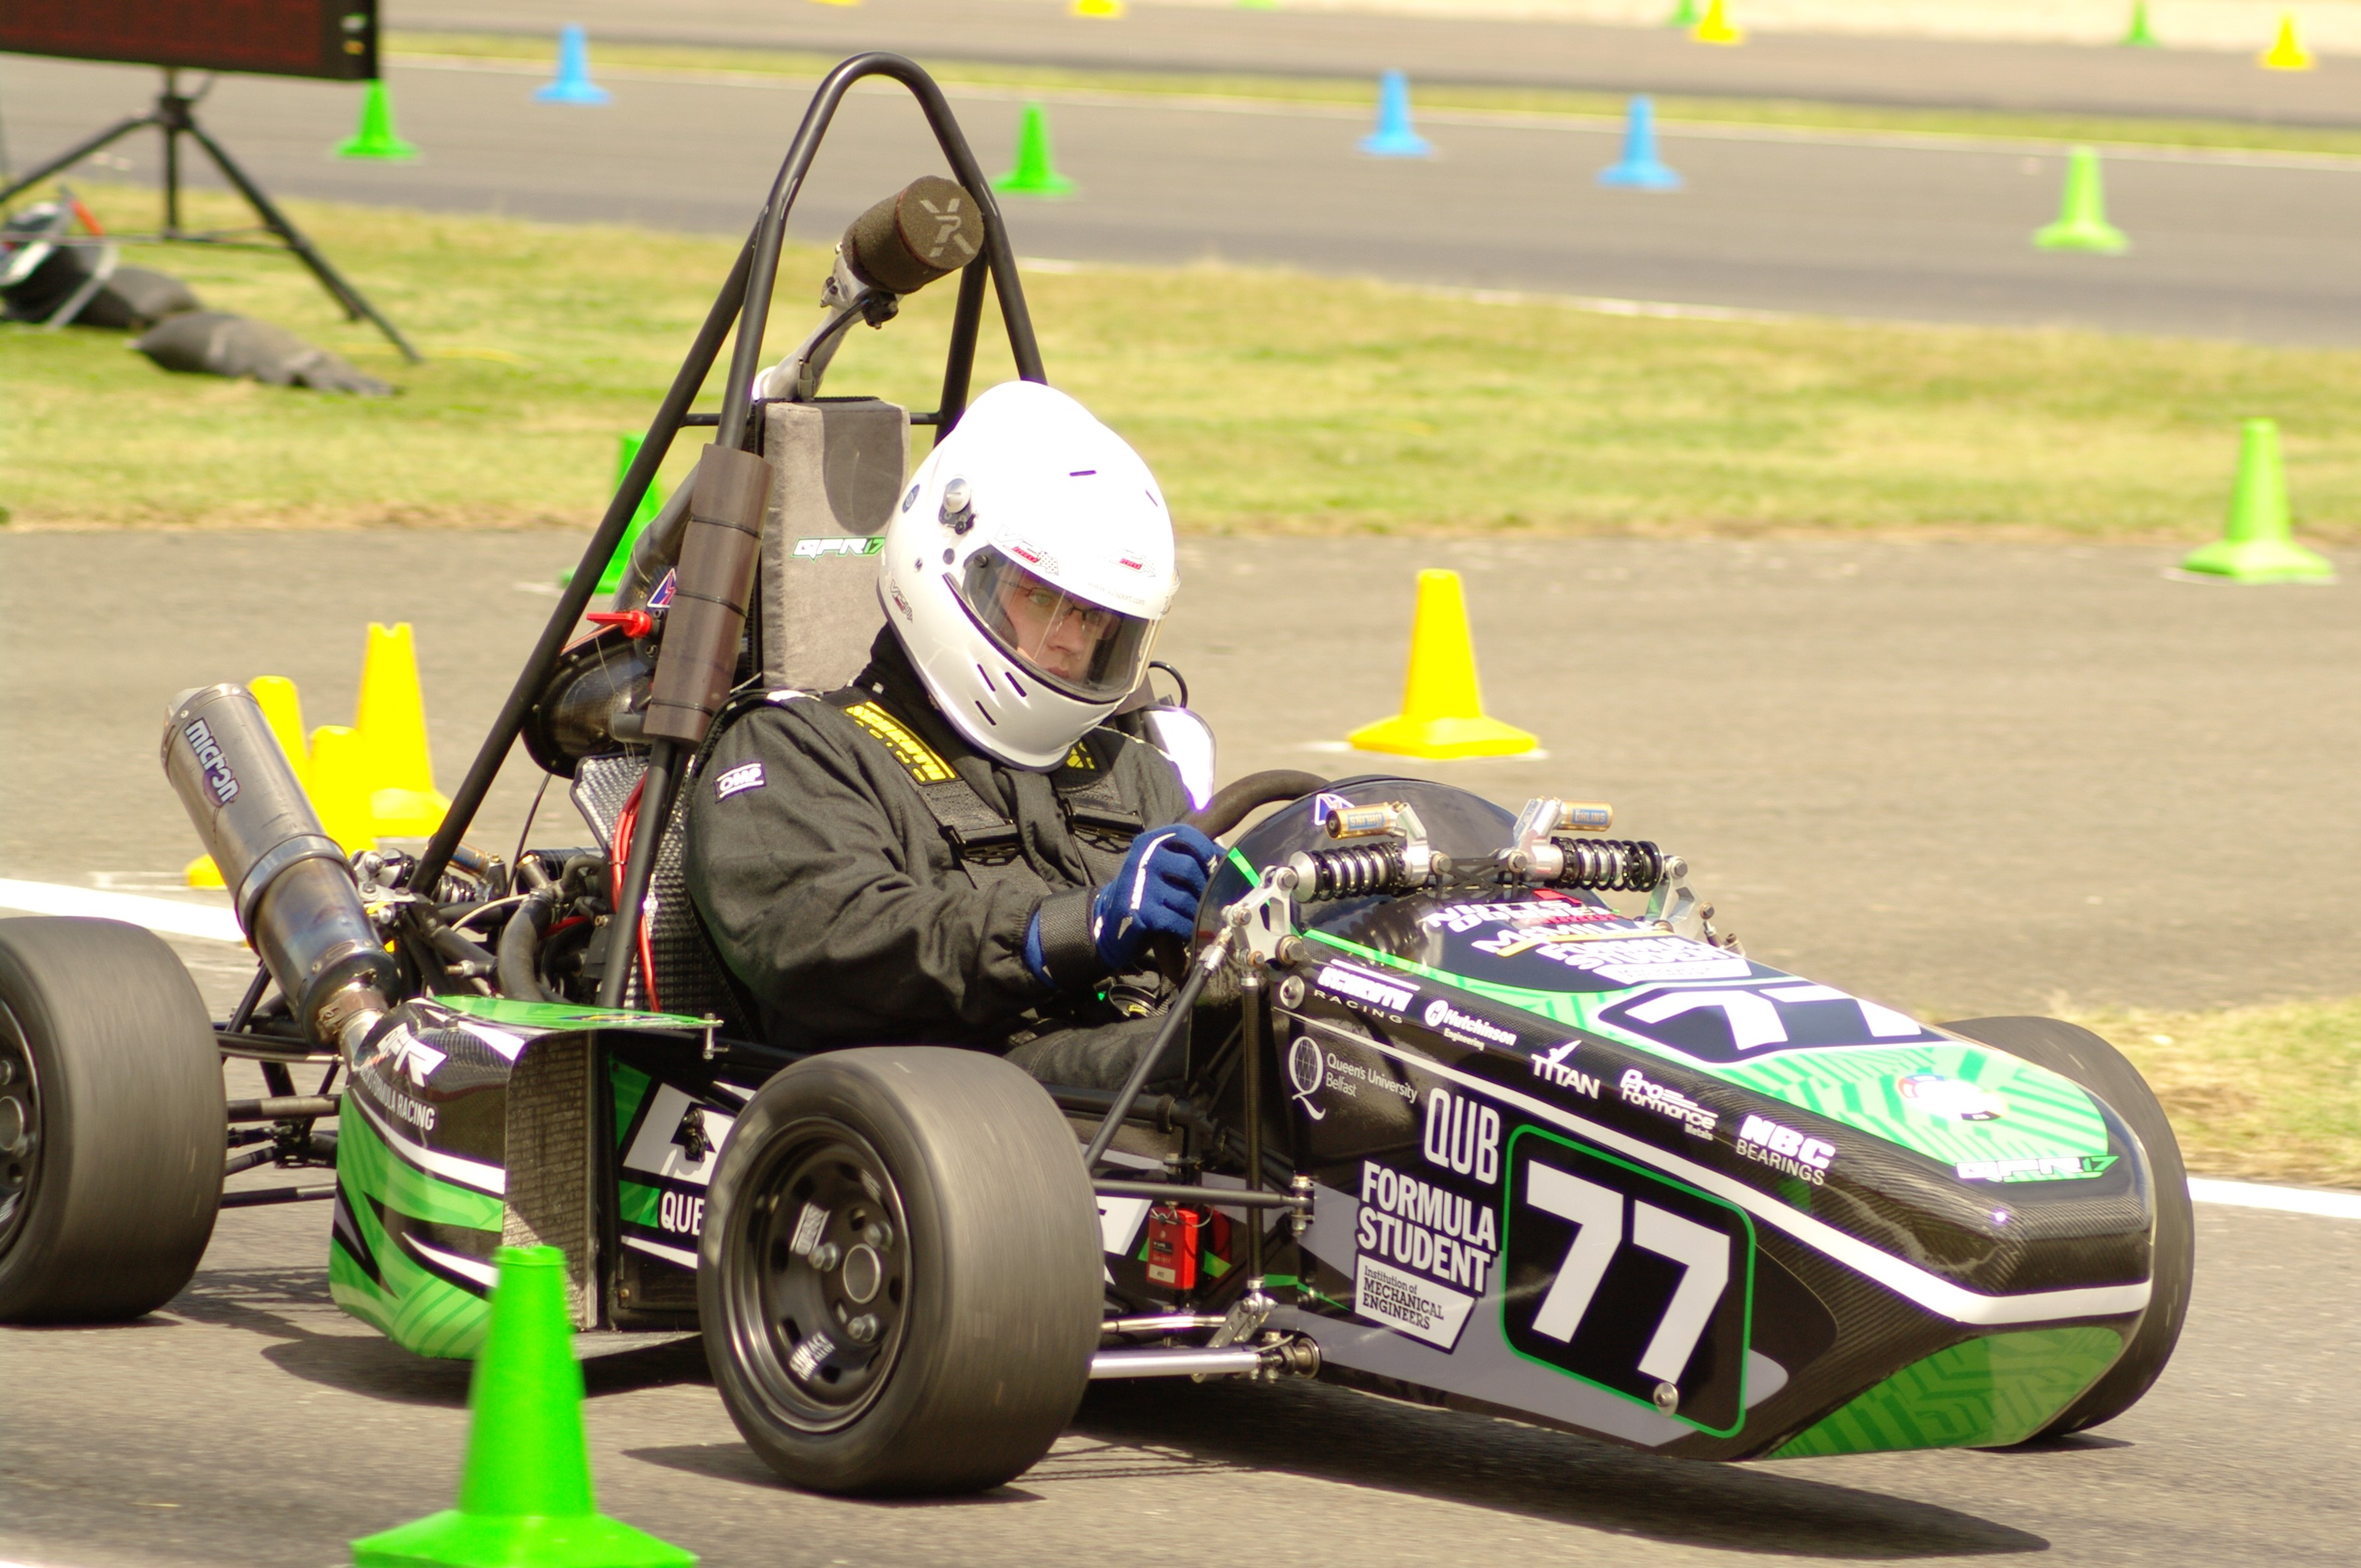
\includegraphics[scale=0.05]{Figures/QFR17PHOTO.JPG}
  \end{subfigure}
  %
  \begin{subfigure}[b]{0.4\textwidth}
    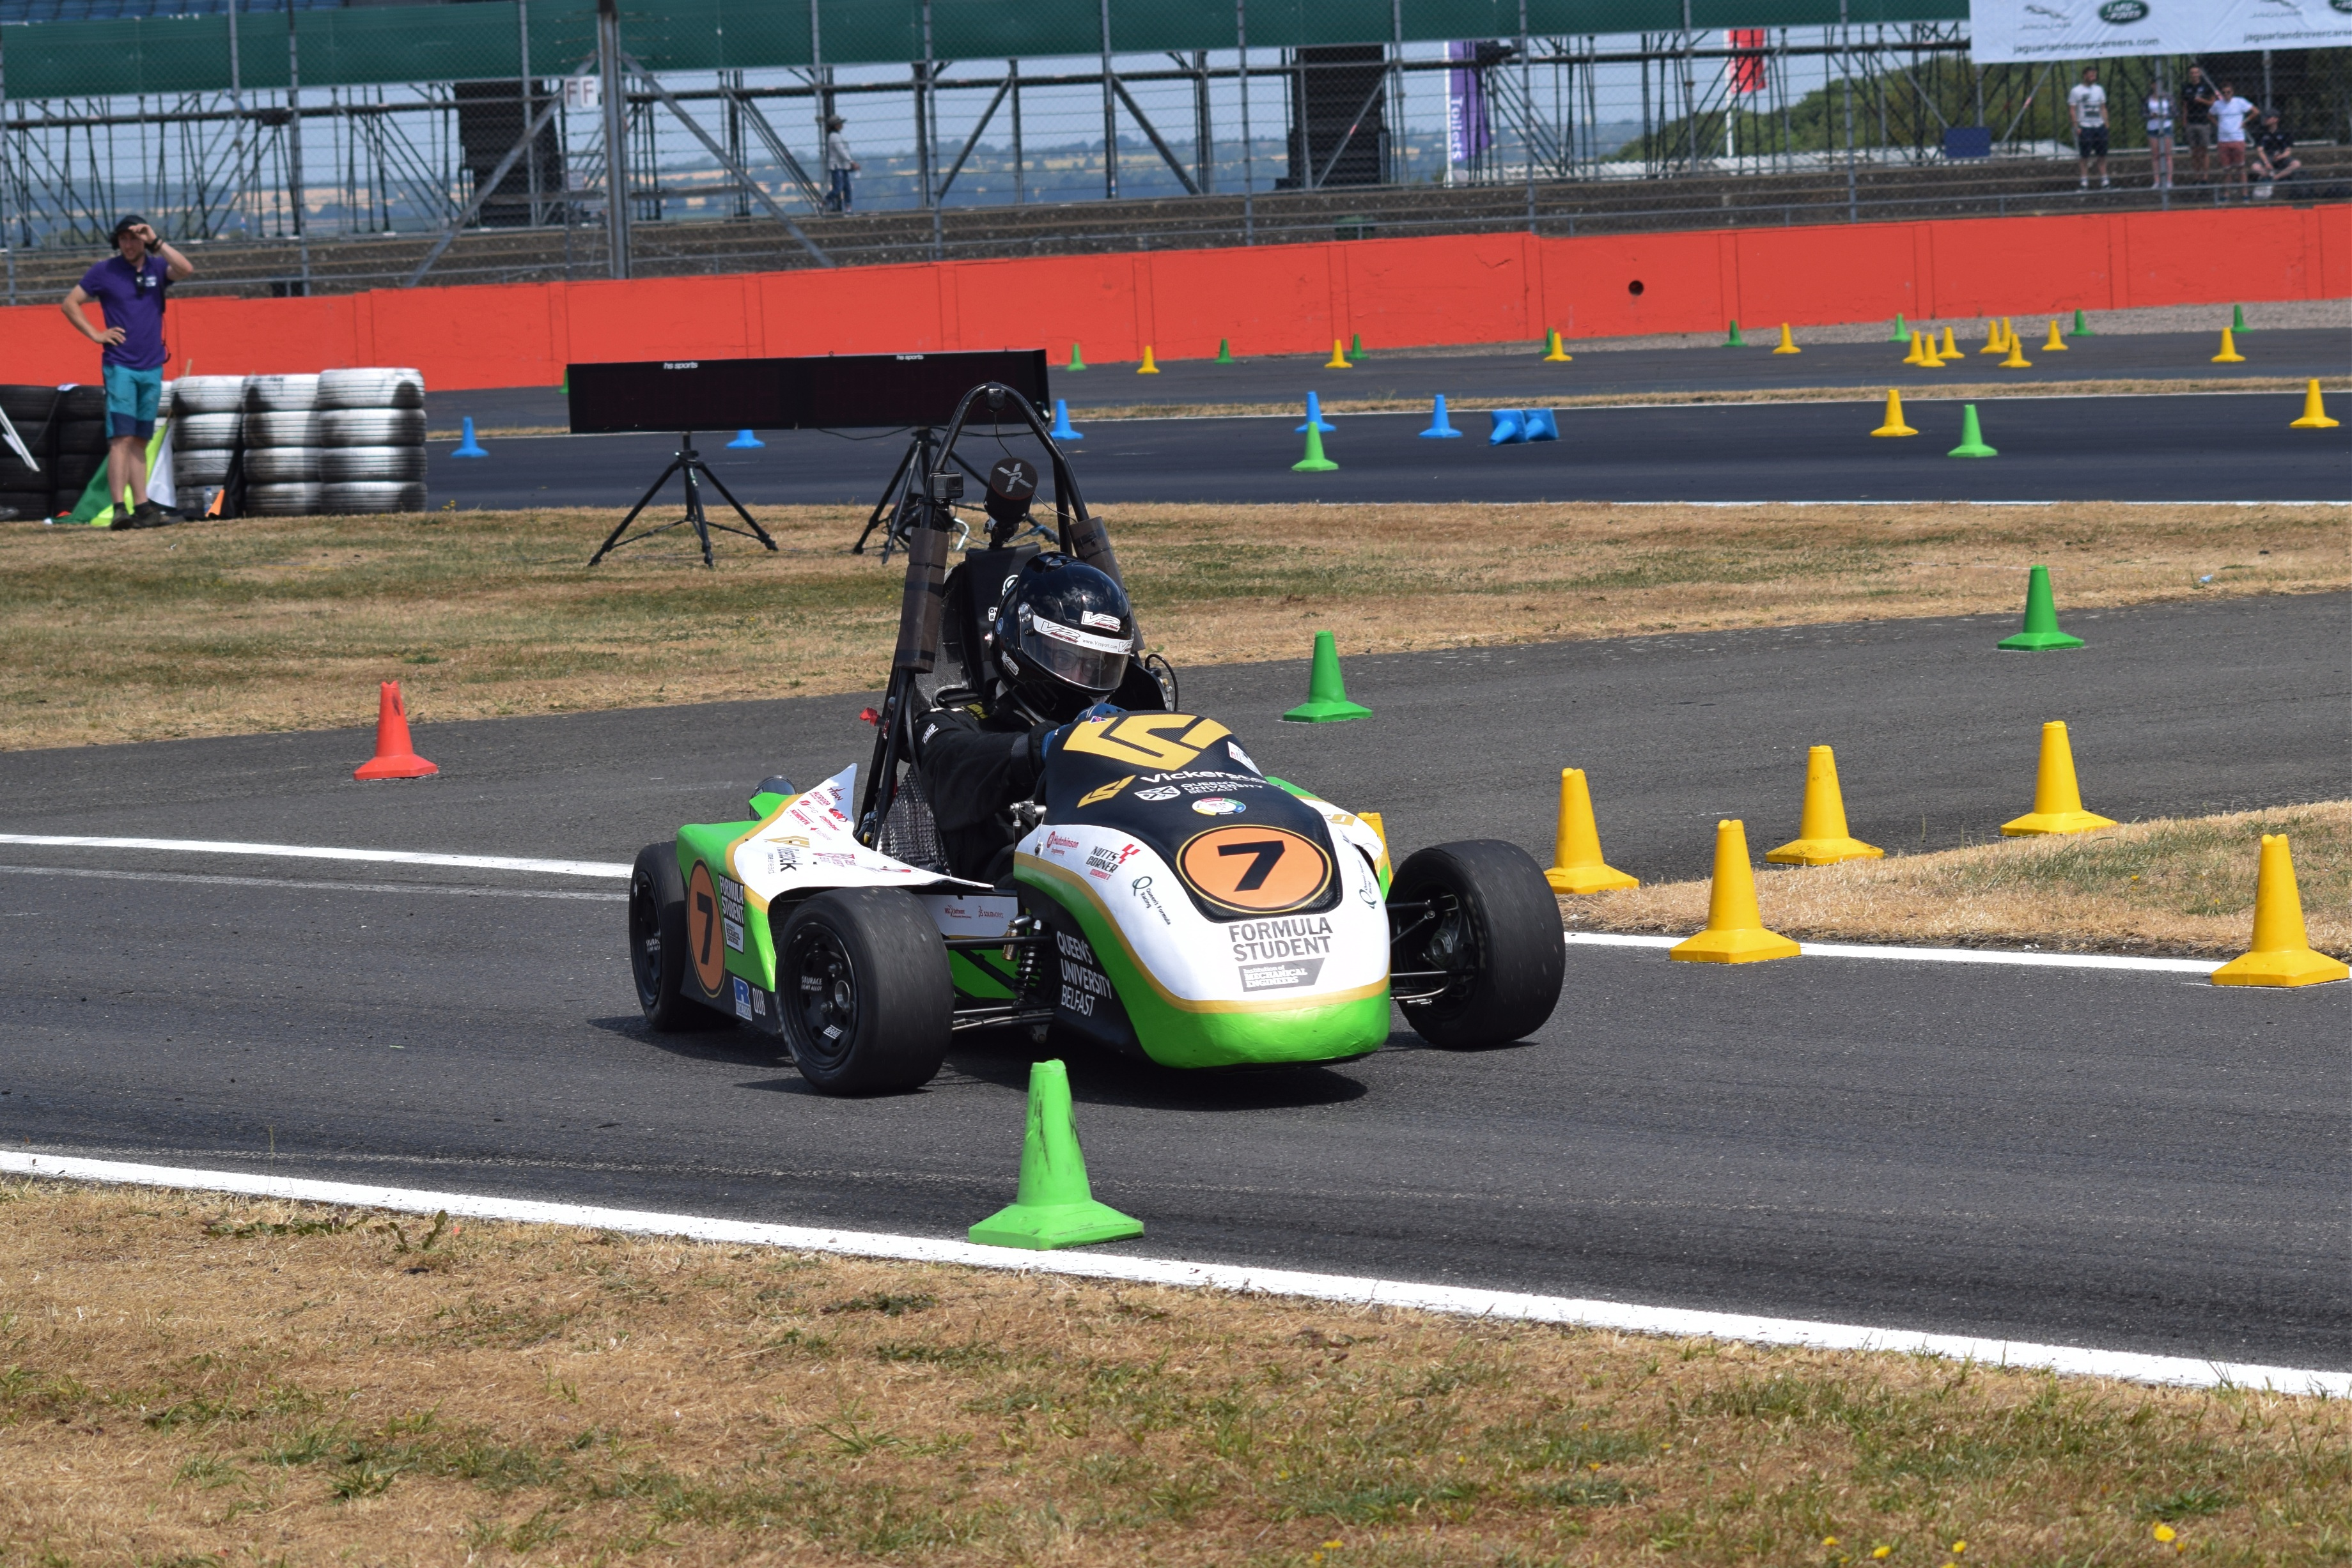
\includegraphics[scale=0.05]{Figures/QFR18PHOTO.jpg}
  \end{subfigure}
%  
  \caption{Queen's Formula Racing car 2017(left) and 2018 (right) on the dynamics event}
    \label{fig:1}
\end{center}
\end{figure}


\noindent Queen's University Belfast is represented by Queen's Formula Racing (QFR) in the event of FSUK since 2007. The team is consisted of undergraduates and postgraduate students which are divided into Engineering sub-teams focusing on chassis, suspension \& unsprung mass, powertrain, electrical, and performance. Consideration of aerodynamic aspect on QFR car was first initiated in 2017 which focus on the aerodynamic analysis framework\cite{Corr2017MechanicalAuthor}. In 2018 the first design of aerodynamics undertray for QFR race car was generated\cite{McKeown2018DesignCar}, and this paper is intended to build up the analyses from previous paper and improve the undertray performance by investigating broader and deeper to the variables which could plausibly enhance the overall car performance.  

\subsection{The significance of Aerodynamics in Formula Industry}
Aerodynamics has become a crucial aspect to the high-speed cars performance. The race-car industry has led the technology innovation by indicating the needs of constant improvements \cite{Zhang2006GroundCars}. Engineers have been trying to modify the car's shape to manipulate and advantages the flow around the body. The role of aerodynamics in improving the race-car performance rose in 1968 when inverted airfoil was introduced to Formula One car, and the research in this area has been growing exponentially ever since. 

%put inverted aerofoil race car photo here

\noindent Downforce(negative-lift) is one of the major aerodynamics key in improving the overall race-car's performance. Downforce or negative lift is force product of the aerodynamics flow around the body. On high-speed ground vehicle, this usually achieved by introducing aerodynamic devices such as wing (inverted wing) and undertray which modify the airflow to the engineering needs \cite{Wright1982TheCars}. In the race-car industry, the primary aim is to maximise the downforce while maintaining the drag at the lowest \cite{Zhang2006GroundCars}, but achieving constant performance at diverse speed and acceleration is equally important.  The size of downforce is significantly affected the breaking acceleration and cornering, hence the cornering speed. Despite the restrictive aerodynamics rules in the competition, optimising the downforce could potentially improve the acceleration which increases the chance to overturn the opponent on a corner. Higher downforce could also increase the top-speed in shorter time that reduces the corner entry and exit time. A ground effect aerodynamics that applied to an open-wheeled car is still an experimental science \cite{Zhang2006GroundCars}, this is due to the complex physics flow that involve turbulent wake, interaction of ground boundary layer, dynamic suspension motion, and many more in which accurate analytical capability (experimental \& computational) is not yet sufficient.

\noindent Nevertheless, computational fluid dynamics (CFD) has improve tremendously with the industry over the years and able to produce an accurate results of forces, flow pattern, etc, in some particular geometry of the car. However, one research paper \cite{Zhang2006GroundCars} stated that diffuser is one part of race car that can be hardly understood, therefore specific variable in generating an undertray geometry is required with careful consideration and assumption on the analysis. 

\noindent In this paper, computational fluid dynamics will be used to understand the trend behaviour of an aerodynamics undertray in 2 dimension and 3 dimension with numbers of nozzle \& diffuser variables such as angle, length, and width. These results then will be used as consideration for the geometry dimension of the final aerodynamics undertray for QFR 2021.

\subsection{Project Aims \& Objectives}
The aim of this project is to design and optimise the aerodynamics undertray for Queen's Formula Racing car which improve the car's overall down-force and drag reduction. Final design of the undertray will be based on the computational simulations and design recommendation from previous QFR analysis. The approved final design then will be manufactured and installed to QFR 2021 for the competition if the workshop time and capacity allows.

\noindent
To fulfill the project aim, there were some objectives made:
\begin{itemize}
    \item Analyse the enclosed and open flow 2D \& 3D analyses with various inlet, outlet, and ground clearance variables  using ANSYS Fluent to identify its effect and trend on the undertray lift and drag. 
    \item Design flexible 3D undertray designs based on the 2D analysis results, which then will again be optimised with additional aerodynamic features on the undertray which will improve the downforce and reduce the drag.
	\item Design the final undertray CAD and choose the material which tailored to car’s dimension and goals, then analyse the weight to drag ratio to pick the best performance and material for the car
    \item Manufacture and fit the undertray for 2021 Queen’s Formula Racing car which then will be judged on the Formula Student competition.
\end{itemize}

%___LIT Review__________________________________%
\section{Literature Review}

\subsection{Motor-sport Aerodynamics}
In 1949 Ludwig Prandtl stated, "The term aerodynamics is generally used for problem arising from flight and other topics involving the flow of air \cite{Anderson2007FundamentalsJr.}". By definition, Aerodynamics is one of the branch in physics which concern and study the interaction of a body and fluid flow stream \cite{Scibor-Rylski1984RoadAerodynamics}. The forces' magnitude and direction occur on a body is a result of the flow interaction which depends on several variables. Some fundamental variables in aerodynamics include flow velocity, temperature, pressure, and density, which further describe the flow physics and characteristic. Drag and lift are the greatest consideration in race-car aerodynamic which will be discussed further on next subsection on this paper.

\noindent Aerodynamics is generally classified into external (flow around  the body) and internal (flow inside the body). This paper will focus on external aerodynamics which focus on the force generation due to the air-stream behaviour around the body of interest. In the automotive industry, external force plays an important part since the overall performance of the car is dependent on the aerodynamics forces created which significantly influence and improve the vehicle shape to its aerodynamics advantage \cite{Scibor-Rylski1984RoadAerodynamics}. Some of the aerodynamics consideration to vehicle's shape influence include large downforce generation, downforce balance between from and rear tyre, and drag minimisation. Table \ref{Table1} shows the effect of downforce to a racing car's acceleration, it can be seen that downforce significantly improve the acceleration time by -1.06 seconds, rate of acceleration by 4.5 $m/s^2$, and power by 124 kilowatt. 

\begin{table}[!ht]
\caption{\label{Table1} Aerodynamic downforce effect of a racing car acceleration \cite{Scibor-Rylski1984RoadAerodynamics}.}
\vspace{-5mm}
\begin{center}
 \begin{tabular}{||c| c| c ||} 
 \hline
 Variables & With Downforce & Without Downforce \\ [0.5ex] 
 \hline\hline
 Time from 0 to 160 $km/h$ & 5s & 6.06s \\ 
 \hline
 Rate of acceleration at 44 $m/s$ & 10.02 $m/s^{2}$ & 5.52 $m/s^2$ \\
 \hline
 Power transferred at 44 $m/s^2$ & 353 kW & 229 kW  \\
 \hline
\end{tabular}
\end{center}
\end{table}

\noindent Queen's Formula Racing has started to focus on aerodynamics since 2016. Previous students have attempted to analyse the previous QFR car including undertray to optimise its overall performance.  This paper will solely focus on external aerodynamics to understand the flow behaviour of a QFR undertray and its force generation, which then the analyses are used for geometry consideration of the aerodynamic undertray.

\subsection{Aerodynamics Fundamental}
To fully understand the flow physics and behaviour of the aerodynamic undertray, there are several fundamental understanding or terminologies of aerodynamics which needs to be firstly understood.

\subsubsection{Flow Types}
The main characteristic of a liquid is the molecule ability to freely move around the space. The movement of liquid molecule to another point in space also requires energy, mass, and momentum to be transferred with it. In this occasion the "transfer phenomena" occurred, where the molecules introduced to viscosity (friction), thermal conduction, and mass diffusion \cite{Anderson2007FundamentalsJr.}. The flow that shows the indication of "transfer phenomena" can be called as viscous flow. On the other hand, the flow condition where the "transfer phenomena" does not occur is known as inviscid flow.

\noindent Some flow such as streamline far from wall can be represented by the inviscid flow. But to capture the aerodynamic behaviour between two near moving wall such an undertray, the viscous flow plays a crucial factor. The shear stress near wall boundaries is occurred by the presence of viscosity which become one of the major source in drag, as well the presence of viscosity allows us to capture flow separation on the high incident geometries. Viscous effect is important consideration in the analysis where the body of interest is purposely designed to generate aerodynamic forces due to the flow such as, airfoil and undertray.

\noindent Another important properties in aerodynamics is density ($\rho$). Compressibility on a flow is fully dependant on the the state of its density at certain speed. Incompressible flow can be referred to a flow with constant density throughout, which usually happen at the region of Mach number less than 0.3. In contrast the region of Mach greater than 0.3 is known as compressible flow where density is variable\cite{Anderson2007FundamentalsJr.}.

\subsubsection{Reynolds Number}
%talk about reybold Number as well how it affects the flow characteristic
Reynolds number is a dimensionless ratio of inertial and viscous forces which used to classify the probability of flow being laminar or turbulent\cite{Rehm2008SituationalMPD}. Mathematically, Reynolds Number can be expressed as:

\begin{equation}
Re = \frac{\rho v d}{\mu} = \frac{inertial force}{viscous force}
\end{equation}

\noindent For low Reynolds number, the flow can be categorised as laminar where the molecules move in a regular, smooth, steady, and no mixing between layer occurred\cite{Obidi2014TheoryVehicles}. In contrast the turbulent flow usually occur at high Reynolds number where the fluid particles travel in random and irregular attitude in which break up the streamline. When the flow is changing from laminar to turbulent, this flow is called transition region. Figure \ref{fig:2} shows the difference in laminar flow with transition to turbulent region near the wall. 

\begin{figure}[!htb]
    \centering
    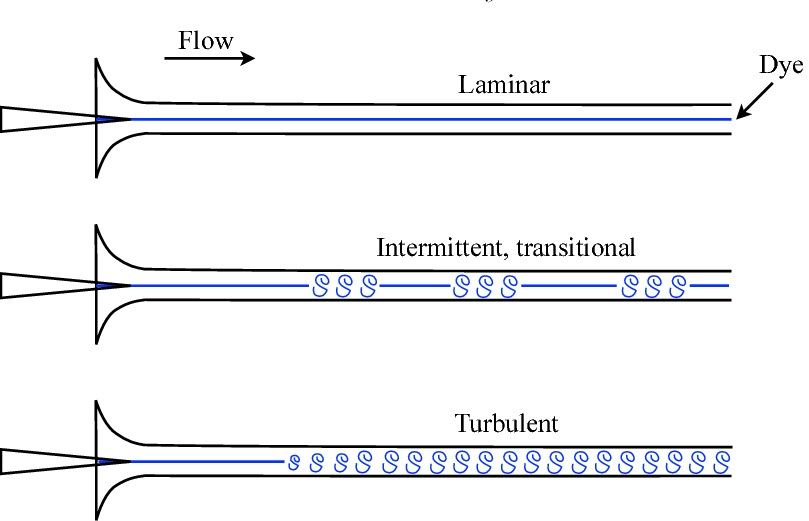
\includegraphics[scale=0.4]{Figures/laminar_turbulent_difference.jpg}
    \caption{Illustration of difference between laminar, transition, and turbulent flow in a pipe \cite{D.BARKLE2016TheoreticalPipe}.}
    \label{fig:2}
\end{figure}

\subsubsection{Boundary Layer}
Boundary layer is the referred as the viscous flow region adjacent to the body surface \cite{Anderson2007FundamentalsJr.}. The layer of air stream surrounding the body at a distance near the wall move with various relative speed, therefore this create a velocity gradient ($\frac{\partial V}{\partial y}$) which the speed on the surface is zero (non-slip condition) to local velocity outside the surface layer \cite{Scibor-Rylski1984RoadAerodynamics}. This layer is also referred as boundary layer. Figure \ref{fig:3} show the development of boundary layer on a flat plate, it started with laminar flow which transitioned into turbulent flow with formation of eddies in it.

\begin{figure}[!htb]
    \centering
    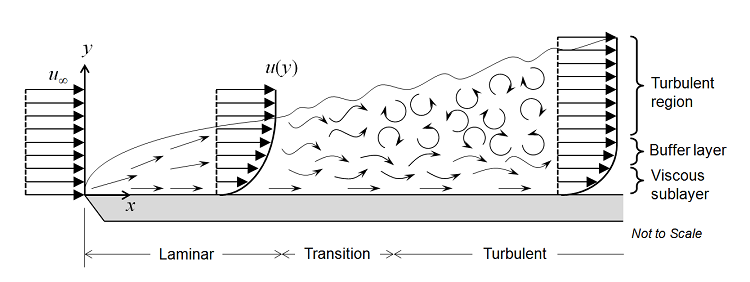
\includegraphics[scale=0.6]{Figures/BL_laminar_turbulent.png}
    \caption{The difference of boundary layer along flat plat \cite{Frei2017WhichApplication}.}
    \label{fig:3}
\end{figure}

 
\noindent From figure \ref{fig:3}, it can be seen that there are two main types of boundary layer flow: laminar and turbulent. Laminar is demonstrated close to the leading edge where the fluid travel smoothly which shows a low velocity gradient and low friction near the wall. When the velocity gradient increases and the friction on one layer to another is significant, the flow can be stated as turbulent \cite{Scibor-Rylski1984RoadAerodynamics}. This can be indicated with irregular and random fluid movement with presence of eddies. Boundary layer is important due to its ability in producing drag due to skin friction. When the local velocity increases, the velocity gradient $(\frac{\partial V}{\partial y})_{y=0} $ and shear stress near the wall ($\tau_w $) also increases with the overall drag.

\noindent It has to be noted that turbulent flow and separated flow are related but different flow characteristic. Flow separation occurs where the air stream effect is reversed when the surface geometry is curving away . When the air stream slows down, the pressure gradient inverses which create an adverse pressure gradient and then cause a thickening in boundary layer \cite{Scibor-Rylski1984RoadAerodynamics}. The condition let the shear stress (friction) and adverse pressure gradient bring the molecules at the very near of the wall come to stop. At this stage the boundary layer separates  and create a region of reversed flow. This condition is illustrated on figure \ref{fig:flow separation}.

\begin{figure}[!ht]
    \centering
    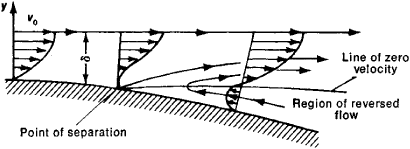
\includegraphics[scale= 0.8]{Figures/flow_separation.png}
    \caption{Illustration of separated flow formation along curved body \cite{Anonymous1979SeparationDictionary}}
    \label{fig:flow separation}
\end{figure}

\subsubsection{Bernoulli Equation \& Venturi Effect}
Bernoulli equation is another important mathematical analysis that analyse the relationship between the flow speed and pressure, this is a fundamental theory of the aerodynamic undertray. The equation can be expressed as:
\begin{equation}
   \underbrace{p}_\textrm{Pressure Energy} + \underbrace{\frac{1}{2} \rho V^{2}}_{\substack{\text{Kinetic Energy} \\ \text{per Unit Volume}}} + \underbrace{\rho g h}_{\substack{\text{Potential Energy} \\ \text{per Unit Volume}}} = constant
    \label{eq:bernoulli}
\end{equation}
Equation \ref{eq:bernoulli} clearly states the relationship between speed and pressure where the flow's density is assumed constant. This states that pressure is inversely proportional to the air speed, therefore increase in velocity has to be accompanied with reduction in pressure and vice versa. This strongly correlated to the downforce generation of an undertray, flow acceleration on the bottom of a car will reduce the pressure, hence high downforce.

\noindent The underbody of a race car can be modelled as a Venturi tunnel where the undertray the airflow goes into area reduction then expanded at the rear which illustrated in figure \ref{fig:venturi_tunnel_car}. The purpose of this shape is to accelerate the flow underneath the body then slowly expanded at the rear diffuser. The continuity formula $\rho AV = constant$ stated the reduction in underbody cross sectional area increases the velocity, hence decreases the pressure (from equation \ref{eq:bernoulli}).

\begin{figure}[!ht]
    \centering
    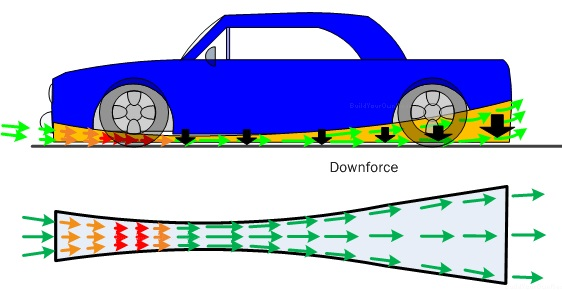
\includegraphics[scale=0.8]{Figures/venturi_tunnel.jpg}
    \caption{Venturi tunnel modelling of an automotive underbody \cite{Anonymous2020RaceDesign}.}
    \label{fig:venturi_tunnel_car}
\end{figure}
\noindent It is worth to be noted that this simplification only applied on ideal condition where the air mass is fully conserved throughout the undertray. In real-life condition, there are some air leakage on the side and creates a corner vortices which greatly affect the overall car performance. The rule of thumb for designers is to maximise the cross-sectional area reduction on the inlet and area expansion on the rear, due to viscosity, this case will not be possible. High area reduction on the inlet will accelerate the flow but also proportional to its drag and high diffuser area (outlet angle) will create flow separation which reduce the downforce and create a significant wake at the rear of the car, hence higher drag. To achieve an optimised underbody geometry, broad variables has to be broadly and deeply analysed to identify each of its effect to the aerodynamic force.


\subsubsection{Aerodynamic Forces}
%due to to flow around the body there are some generation of force occurred etc
Forces optimisation which generated by the aerodynamic flow are the main goal of this paper. The Bernoulli Equation from section 2.2.4 indicated that the flow pattern around a body produces pressure distribution over the surface \cite{Scibor-Rylski1984RoadAerodynamics}, which means integrating the pressure over the body surface will result in total forces caused by the flow around the body. The general force of a body can be expressed as:
\begin{equation}
    F = qSC_f
\end{equation}
Where $C_f$ is a dimensionless coefficient which fully dependant on the shape of the body \cite{Scibor-Rylski1984RoadAerodynamics} and $S$ is the area on which the surface the force of a body. In a drag analysis, the surface is the frontal area of a body which imposed the flow velocity (illustrated on figure \ref{fig:Force direction and frontal area} right). On the other hand, the lift analysis will require the area of the lift generator (e.g. undertray, inverted wing, or car wetted-surface).

\begin{figure}[!h]
\begin{center}
%    
  \begin{subfigure}[b]{0.4\textwidth}
    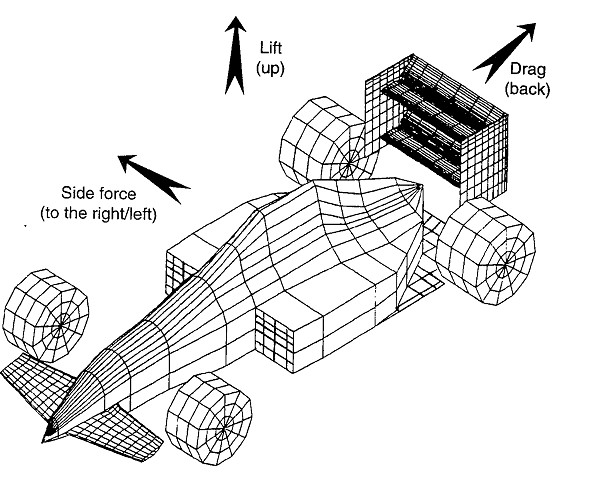
\includegraphics[scale=0.4]{Figures/race_car_forces.jpg}
  \end{subfigure}
  %
  \begin{subfigure}[b]{0.4\textwidth}
    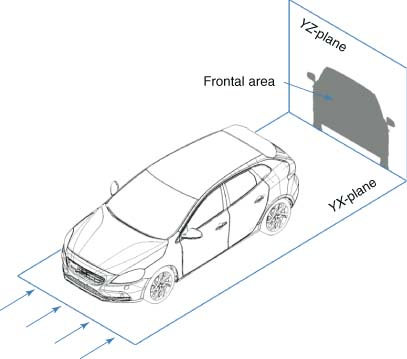
\includegraphics[scale=0.8]{Figures/frontal_area.jpg}
  \end{subfigure}
%  
  \caption{Force direction acting on a race-car(left) and representation of frontal area of an automotive body(right)\cite{Sebben2014FundamentalsDesign}.}
    \label{fig:Force direction and frontal area}
\end{center}
\end{figure}
\noindent There are three main forces acting on a car body: lift, drag, and side force. Figure \ref{fig:Force direction and frontal area} left illustrate the direction of forces acting on a car. Due to the function of undertray, this paper will only focus on the generation and optimisation of lift and drag.

\paragraph{Lift (downforce)}
%definition of lift
Lift is an applied force due to the pressure difference on a body which acts vertically and perpendicular to the drag force \cite{Scibor-Rylski1984RoadAerodynamics}. It can be mathematically expressed as:
\begin{equation}
    L = \frac{1}{2}\rho U^2 S C_L
\end{equation}
%lift in race car 
It is important in motor-sport industry that a race car produce as much downforce (negative lift) with the least drag possible. In aviation field, the aerofoil generate positive force to lift the aircraft from the ground, on the other hand, lift on race car used to increase the tyre grip by using an inverse aerofoil concept which produce a negative force. This consideration is due to the significant improvement in road handling and tyre grip which enables higher cornering speed, acceleration, and braking \cite{Barnard1997RoadIntroduction}.


\paragraph{Drag}
Drag is a force that work against the intended direction of a body which manifest in form of friction or pressure\cite{Obidi2014TheoryVehicles}. The drag force direction always follows the flow velocity of the car motions. Drag force can be mathematically expressed as:
\begin{equation}
    D = \frac{1}{2}\rho U^2 S C_D
\end{equation}
In case of formula student car, the flow travels around the car can be assumed as stokes flow (low Reynold number flow) which stated that drag is directly proportional to the viscosity, velocity, and size \cite{Obidi2014TheoryVehicles}. If the viscosity of air can be assumed as constant in the analysis, therefore the only variable which could be modified to reduce the drag is the size or geometry of the body. It has to be noted that race-car drag also divided into 5 different type of drag \cite{Kelly1964AerodynamicsEngineers}: form drag, lift drag, surface drag, interference drag, internal flow drag.

\subsection{Aerodynamics Undertray}
Undertray is an aerodynamics device that is attached to the underside of a race car that take advantages of the aerodynamic flow to decreases the pressure and increase the downforce significantly. Undertray has become an important part in motor-sport industry due to its ability to produce 45\% of car's downforce \cite{Katz1995RaceSpeed}. A typical undertray consist of a nozzle (inlet), floor section (throat), and diffuser (outlet).  Figure \ref{fig:underbody} shows an example of simple undertray of a formula car.

\begin{figure}[!ht]
\begin{center}
%    
  \begin{subfigure}[b]{0.4\textwidth}
    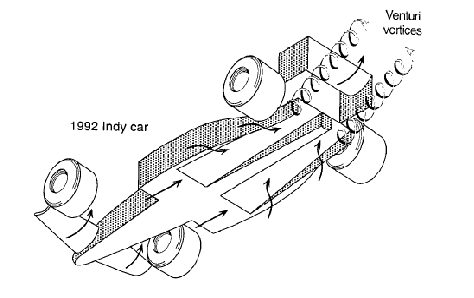
\includegraphics[height=4.8cm]{Figures/underbody.PNG}
  \end{subfigure}
  %
  \begin{subfigure}[b]{0.4\textwidth}
    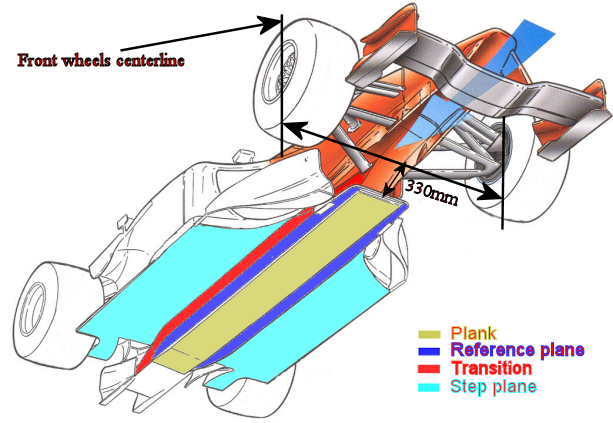
\includegraphics[height=4.8cm]{Figures/undertray_f1.png}
  \end{subfigure}
%  
  \caption{Typical undertray of a formula race-car \cite{Katz1995RaceSpeed}\cite{AnonymousUndertrayUnderbody}}
    \label{fig:underbody}
\end{center}
\end{figure}

\noindent As stated before, the concept of Venturi tunnel is used for an undertray to generate downforce. the convergent section of the Venturi tunnel allows the increase in velocity which reduce the pressure on the floor section. A significant pressure reduction create a suction-like phenomena which push the car down and create a higher traction. On the rear side of the undertray is the divergent section (diffuser) where kinetic energy is converted into a pressure rise. 
\noindent Up to QFR 2021, undertray is the only passive aerodynamics device which will be produced and attached to the car. The development of undertray of QFR 2021 has been done previously in 2017 \cite{McKeown2018DesignCar} and 2019 \cite{McClune2018DesignCar}. The work has included a numbers of 2D simulations which tested various variables of the undertray such as diffuser and inlet angle, as well some of 3D undertray. The case analyses by McKeown \cite{McKeown2018DesignCar} and McClune \cite{McClune2018DesignCar} was flawed due to the non-existence of bluff body. This allows the analysis on the undertray force generation affected by the flow acting on the top of the undertray which makes the analyses unrealistic to the real-life situation \cite{Corr2017MechanicalAuthor}. Therefore this paper will dig deeper on the flow behaviour of the underbody with bluff body both on 2D and 3D analyses. 

\subsubsection{Undertray Devices}
The geometry design of an undertray is strictly regulated by the competition. Although Formula students rules is more flexible, there are some device implementation in formula car that could slightly improve the aerodynamics performance. Such devices are diffuser fences and Gurney flaps.

\begin{figure}[!ht]
\begin{center}
%    
  \begin{subfigure}[b]{0.4\textwidth}
    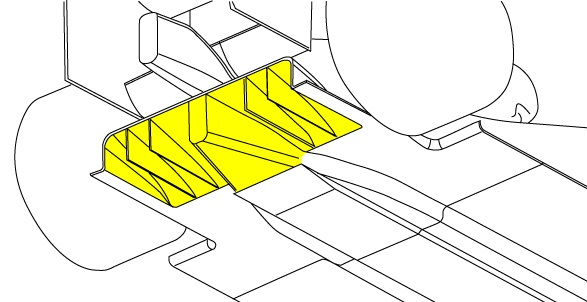
\includegraphics[scale=0.6]{Figures/diffuser_fences.jpg}
  \end{subfigure}
  %
  \begin{subfigure}[b]{0.4\textwidth}
    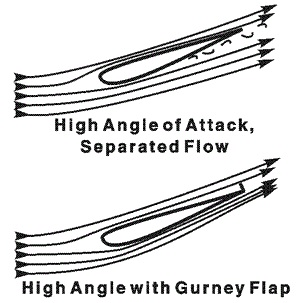
\includegraphics[scale=0.8]{Figures/Gurney.jpg}
  \end{subfigure}
%  
  \caption{Fences or strake on a diffuser(left) and example of a Gurney flap application on a wing (right) \cite{Anonymous2020GurneyFlap}.}
    \label{fig:gurney}
\end{center}
\end{figure}

\noindent Fence or strake on a diffuser acts as a force generator. As discussed previously, the corner vortices occurred at rear diffuser generates downforce and strake helps the diffuser to generate more than two vortices hence increase more downforce. Figure \ref{fig:gurney} left shows the example of a basic strake on a diffuser. Gurney flap is an small flap or L-shape structure attached at the end of diffuser which shown in figure \ref{fig:gurney} right. Generally, Gurney flap is used to improve downforce without significant drag \cite{Willemsen2012CFD-basedDiffuser} by making the boundary layer stay attached and delay flow separation to the end of diffuser by reducing the pressure on the underside of diffuser and increasing the pressure on the top of diffuser. 

\noindent Despite the advantageous function of both device, there are still lack of information provided in this area hence further analysis will be a good leap in improving an undertray performance.  


%___Methodology__________________________________%
\section{Methodology}
To understand the flow behaviour in various undertray geometries, some kind of analysis of the fluid dynamics is required. The rapid development of computational power has allowed more accurate and reliable computational analysis results such as computational fluid dynamics (CFD) \cite{Andersson2011ComputationalEngineers}. The usage of CFD allows engineers to simplify design processes and to achieve an accurate flow prediction in a relatively short period of time, allowing engineers to do more design iterations and thus produce better designs.

\begin{figure}[!htb]
    \centering
    \makebox[\textwidth]{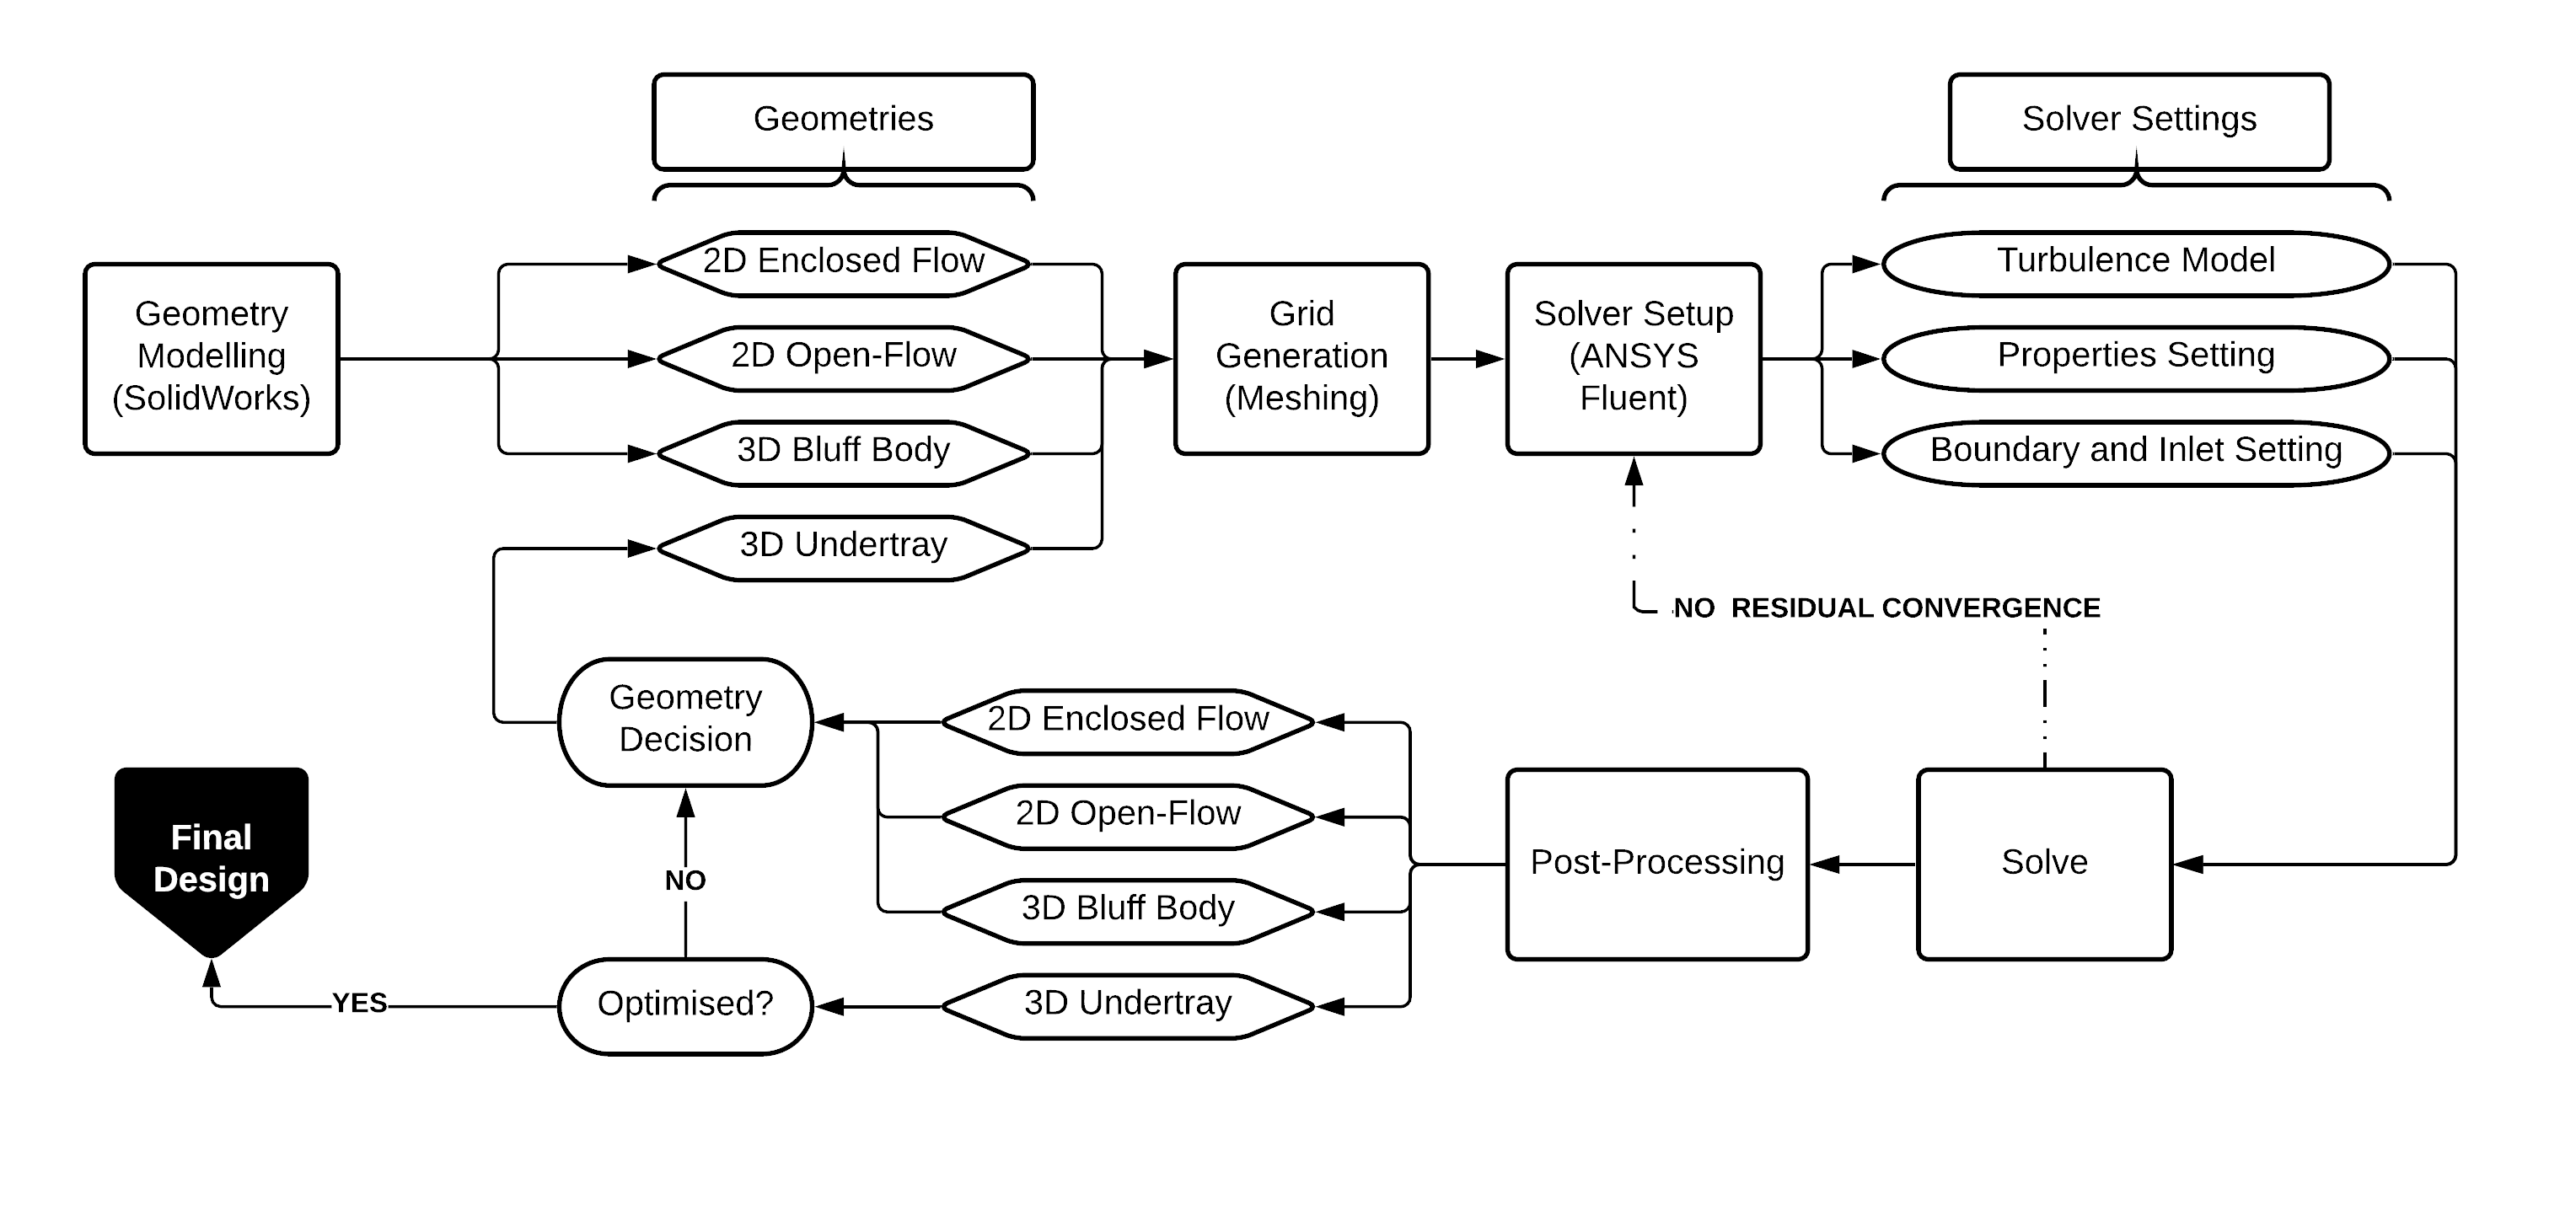
\includegraphics[scale=0.15]{Figures/project_methodology_chart.png}}
    \caption{Project Methodology Flow Chart}
    \label{fig:project methodology}
\end{figure}

\noindent The methodology used in this project consists of three phases. These phases are: 2D enclosed \& open-flow; 3D bluff body flow, 3D full undertray flow. The first phase consists of 2D analysis, which analyses the undertray variables on a Venturi-tube like geometry, and open-flow analysis to determine the effect of a simple bluff body with similar undertray variables. The 3D bluff body phase takes the 2D geometry, extrudes it into a 3D geometry, and then analyses it. Lastly is the 3D full undertray, in which the results from previous analysis will be used to optimise the final undertray design's geometry. A simplified traced body from the QFR 2021 car will be attached to the undertray to achieve results without the geometrical complexity of the full CAD model. The full workflow of the process is illustrated in Figure~\ref{fig:project methodology}. This project will be entirely computationally based, and makes use of ANSYS Fluent as the default working platform.

\subsection{Pre-Processing \& Solver Setup}

\subsubsection{Grid Generation (Meshing)}
\noindent The surfaces or bodies which have been defined from the SolidWorks CAD model forms the basis for the meshing. The meshing program, which is integrated with ANSYS Workbench, provides a user-friendly, simple, and fast mesh generator. Due to the constraints on computational power and time, unstructured triangular (2D) and tetrahedral (3D) mesh were mostly used, with quadrilaterals (2D) and triangular prisms (3D) used near the wall as an inflation layer to capture the growth of the boundary layer and reduce numerical diffusion \cite{Lanfrit2005BestFLUENT}.

\noindent The goal of the 2D and 3D bluff body simulations is to obtain and analyse the trend in performance resulting from changes to the undertray geometry; therefore, a simple yet high quality mesh could be generated in an unstructured manner. Local refinement around the solid body is recommended \cite{Lanfrit2005BestFLUENT} to achieve reasonable results and representation of the flow, especially around the undertray. Moreover, this technique allows reduced mesh density in the far-field sections less likely to be affected by or affecting the result. Another aspect of quality meshing is the mesh metrics such as skewness and growth ratio. For automotive applications, it is recommended to have skewness less than 0.45 and a maximum growth rate of less than 20\% \cite{Lanfrit2005BestFLUENT}. 

\noindent One crucial factor in an undertray flow is the development of the boundary layer, and how this interacts with the moving floor. The accuracy of this aspect is dependent on the quality of the grid near the wall, and on the wall function being used. To generate a high quality inflation layer, it is essential to make sure the y+ value (first layer grid height) does not exceed the inner boundary layer region, which can be calculated using the expression:

\begin{equation}
    y^+ = \frac{\rho U_\tau y}{\mu}, where \quad U_\tau = \sqrt{\frac{\tau_w}{\rho}} = U \sqrt{\frac{1}{2}C_f}
\end{equation}

\noindent The turbulence model being used by the solver also has to be considered in defining the required $y^+$ value. Some turbulence modelling requires a very low $y^+$, whereas some can tolerate higher values. The detail of $y^+$ value in the various turbulence models will be discussed in the next section. 

\subsection{Numerical Method}
\label{section: Numberical Method}
\noindent The turbulence model is a crucial aspect in approximating the effect of unsteady turbulent fluctuations on the flow \cite{Cummings2015AppliedAerodynamics}. The quality of the turbulence modelling can significantly impact the fidelity of the simulations \cite{Lanfrit2005BestFLUENT}. Due to the time constraints and limited computational resources available for this project, a steady-state method was used throughout. To account for the effects of turbulence, a two-equation Reynolds-Averaged Navier-Stokes (RANS) approach was used to solve the time-averaged flow \cite{Cummings2015AppliedAerodynamics}. With a reasonable quality of mesh, physical lift and drag trends can be predicted, which can then be studied. The Realizable $k-\epsilon$ and $k-\omega$ Shear Stress Transport (SST) models were used in this project to solve the equations and estimate the downforce and drag of the undertray and bluff body.  

\subsubsection{Realizable $k-\epsilon$ Models}
The $k-\epsilon$ turbulence model is a two-equation transport model which specifically solves equations for the turbulence kinetic energy ($k$) and turbulence dissipation rate ($\epsilon$) \cite{Andersson2011Turbulent-flowModelling}\cite{Mansour1989Near-wallModeling}\cite{Ansys2006ModelingFlows}. The standard model is robust and widely used across a broad swathe of applications in engineering turbulence modelling; however, the nature of $k-\epsilon$ family is not able to calculate some of the $\epsilon$ terms which can be anticipated using wall function. Moreover, k-$\epsilon$ does not perform well for flow with strong separation and large adverse pressure gradient, which the primary feature of an undertray's diffuser \cite{Ansys2006ModelingFlows}.  Therefore realisable k-$\epsilon$ is broadly used in this analysis. The term 'realisable' itself allows some of the mathematical satisfaction in computing the Reynolds stresses, improving its turbulent flow consistency. This specific transport model is crucial to capture important flow features of an undertray, such as flow rotation, significant adverse pressure gradient, and vortex formation.
\begin{align}
\frac{\partial}{\partial t}(\bar{\rho} k)+\frac{\partial}{\partial x_j}(\bar{\rho} \tilde{u}_j k) & = \frac{\partial}{\partial x_j} \left[ \left(\mu + \frac{\mu_t}{\sigma_k}\right) \frac{\partial k}{\partial x_j} \right] +P_k-\bar{\rho}\epsilon \\ 
\frac{\partial }{\partial t}(\bar{\rho} \epsilon)+\frac{\partial}{\partial x_j}(\bar{\rho} \tilde{u}_j \epsilon) & = \frac{\partial}{\partial x_j} \left[ \left(\mu + \frac{\mu_t}{\sigma_{\epsilon}}\right) \frac{\partial \epsilon}{\partial x_j} \right] + \frac{\epsilon}{k}(C_{\epsilon 1}P_k-C_{\epsilon 2}\bar{\rho} \epsilon),
\end{align} 

\subsubsection{$k-\omega$ Shear Stress Transport (SST) Models}
The SST model is another two equation-model. It combines both the $k-\epsilon$ and $k-\omega$ models \cite{Andersson2011Turbulent-flowModelling}\cite{Ansys2006ModelingFlows}.  The $k-\epsilon$ approach is used in the free-stream, and $k-\omega$ is used near the boundary surface, meaning that this model takes the strength of, theoretically allowing accurate predictions in all regions. This model is known to perform well in regions with adverse pressure gradients and with flow separation; moreover, SST is known to have more accurate performance in the boundary layer compared to $k-\epsilon$ and does not require any wall function\cite{Andersson2011Turbulent-flowModelling}. However, a fine mesh ($y^+  < 5$) is required near the wall, which increases the computational cost and time, and it can over-predict turbulence levels flow in high strain areas \cite{Andersson2011Turbulent-flowModelling}\cite{Ansys2006ModelingFlows}. \begin{align}
\frac{\partial }{\partial t}({\rho} k)+\frac{\partial}{\partial x_j}({\rho} {u}_j k) & = \frac{\partial}{\partial x_j} (\Gamma_{k} \frac{\partial k}{\partial x_j}) + \tilde{G_k} - Y_k +s_k \\
\frac{\partial}{\partial t}(\rho \omega)+\frac{\partial}{\partial x_j}({\rho} {u}_j \omega) & = \frac{\partial}{\partial x_j}(\Gamma_\omega \frac{\partial \omega}{\partial x_j}) + G_\omega - Y_\omega + D_\omega + S_\omega
\end{align} 

\subsection{Boundary Conditions}

\begin{table}[!htb]
\centering

\caption{Boundary Conditions for 2D and 3D ANSYS Fluent Setup.}
    \label{tab:Boundary Conditions}

\begin{tabularx}{0.95\textwidth}{ 
  || >{\centering\arraybackslash}X 
  | >{\centering\arraybackslash}X
  | >{\centering\arraybackslash}X ||
  }
  
  \hline
  Named Region & Boundary Conditions & Property Details \\
  \hline
  \multicolumn{3}{||>{\hsize=\dimexpr3\hsize+3\tabcolsep+\arrayrulewidth\relax\centering}X||}{General Properties}\\
  
  
  \hline
  Inlet & Inlet Velocity & Velocity = 16.667 $m/s$ (or 40 $km/h$) \\
  \hline
  Outlet & Outlet Pressure & Gauge Pressure = 0 Pa \\
  \hline
  Undertray (2D Enclosed) / Bluff Body & Stationary Wall & No-Slip Condition \\
  \hline
  Moving Floor & Moving Wall & Velocity = 16.667 $m/s$ or 40 $km/h$ In the Flow Direction\\
  \hline
  \multirow{4}{*}{Enclosure} & \multirow{4}{*}{Fluid (Air)} & Pressure = 101325 Pa\\
  && Temperature = 288.15 K\\
  && Density = 1.225 $\frac{kg}{m^3}$\\
  && (ISA Sea Level Condition)\\
  \hline
  
  \multicolumn{3}{||>{\hsize=\dimexpr3\hsize+2\tabcolsep+\arrayrulewidth\relax\centering}X||}{3 Dimensional Analyses}\\
  \hline
  Symmetry Body & Symmetry & - \\
  \hline
  Symmetry Top & Symmetry & - \\
  \hline
  Symmetry Side & Symmetry & - \\
  \hline
  
\end{tabularx}
\end{table}
  

\noindent Table \ref{tab:Boundary Conditions} shows the boundary conditions that were used for both the 2D and 3D analyses in the ANSYS Fluent solver. The main goal of these simulations is to simulate the flow behaviour at the bottom region of the car; therefore, a moving floor was employed in all simulations, with the same magnitude and direction as the oncoming flow. The use of a moving ground condition (or a belt in a wind tunnel) is physically correct, and represents the best option for capturing the ground effect in such an undertray \cite{Zhang2006GroundCars}\cite{Burgin1986WINDEFFECT}. The simulation environment was set from the International Standard Atmospheric (ISA) conditions at sea level. 

\noindent In the three dimensional simulations, the side, far-side, and the top surface of the flow-field were set to symmetry conditions, in which the fluxes and normal gradients of all the variables are assumed zero \cite{ANSYS2009SymmetryConditions}, as recommended by Lanfrit \cite{Lanfrit2005BestFLUENT}. Along with the moving floor, this setup was considered to provide the best results and nearest approximation to simulating the behaviour of a race car on an actual racing track.







%___Results__________________________________%
\newpage
\section{2Dimensional Analyses}
This section will discuss the trend and effect of various undertray variables in 2 dimension. The variables tested consist of inlet angle, outlet angle, \& ground clearance which the optimised value will be used for 3 dimensional undertray analysis. The 2D analysis will consist of Enclosed flow analysis which use the Venturi-tube like geometry to simulate the flow of the undertray, and open-flow analysis which use the bluff body to simulate the flow behaviour and interaction between undertray and the bluff body. 

\subsection{2D Enclosed Flow}



\end{document}
